\chapter{Installing \textbf{Andika!}}
\renewcommand{\thesection}{A/\arabic{section}}  % redefine the section numbering
\setcounter{section}{0}  % reset counter
\label{appA}


\begin{quotation}
\begin{small}
\noindent I am grateful to Natalie Kontny, Student Assistant on Project C07, \textbf{The Place of Swahili Manuscripts in East African Collections},  at the University of Hamburg's Centre for the Study of Manuscript Cultures,\footnote{\url{www.manuscript-cultures.uni-hamburg.de/Projekte_e.html}} for road-testing these instructions and helping to write them up.                                                                                                                                                                                                                                                                                                                                                                         \end{small}
\end{quotation}


\section{How much of this do I need to do?}

If you simply wish to be able to type Swahili in a word-processor, you need not go through the full installation procedure in this appendix.  After installing Ubuntu, you only need to follow \Cref{s:snapshot}, move into the unzipped download, and then follow \Crefrange{s:fonts}{s:libreoffice}.

However, if you wish to transcribe, edit and annotate Swahili documents in Arabic script, providing Roman equivalents as well, then you will need to carry out the full installation procedure here.  The reason there is so much to install is that \textbf{Andika!} tries not to reinvent the wheel -- rather, it combines already-existing best-of-breed software to do new things.

Most of the install is carried out by typing in commands directly.  This is because this method is much faster and more succinct than explaining how to point-and-click through various dialogue boxes.


\section{Ubuntu Linux}

\textbf{Andika!} was developed on Ubuntu 14.04,\footnote{\url{ubuntu.com}} a variety of GNU/Linux,\footnote{\url{en.wikipedia.org/wiki/Linux}} a secure and free operating system.  ``Free'' here means not only that it is available at no cost (free as in beer), but also that the user is free to copy, change and distribute it without fear of copyright lawsuits (free as in freedom).\footnote{\url{fsf.org}}  Ubuntu is a user-friendly packaging of a wide variety of software which is suitable for any computing need -- the name is a Southern Bantu cognate of the Swahili \textbf{utu}, and means ``humanity'' or ``humanness'': it is intended to emphasise that the free software concept of sharing brings out the best in all of us.

You can download the current 64-bit\footnote{Most modern machines should be 64-bit capable.} version of Ubuntu 14.04 from \url{http://www.ubuntu.com/download/desktop}\footnote{Although versions such as 15.04 are now available, it is best to stick to 14.04, since this is a Long Term Support release which will be supported for 5 years.}  You can install Ubuntu as the sole operating system on a computer (highly recommended),\footnote{\url{ubuntu.com/download/desktop/install-ubuntu-desktop}} or install it alongside an existing operating system so that you can ``dual-boot'' into either operating system.\footnote{Doing an internet search on ``dual-boot Ubuntu'' should produce a number of guides, such as the one at \url{linux.about.com/od/LinuxNewbieDesktopGuide/ss/The-Ultimate-Windows-81-And-Ubuntu-Dual-Boot-Guide.htm}}

Another possibility is to run Ubuntu inside your existing operating system, as a ``virtual machine''.  This will work well on most machines, though there may be issues with some, and it is always less efficient than running Ubuntu directly ``on the metal''.  Notes on installing a virtual machine are in \Cref{s:ubuntuvm}.


\section{Conventions}

Unless otherwise indicated, lines in\\
\texttt{monospaced font}\\
are commands to be typed in.  

Unless otherwise indicated, all commands should be activated by pressing \textbf{Return} at the end of the command.

The symbol $\hookrightarrow$ at the beginning of a line means that it is a continuation of the previous command, and therefore \textbf{Return} should only be pressed after the end of this line.

Keys separated by + should be pressed simultaneously.  Thus \textbf{Ctrl+X} means ``press the Ctrl key at the same time as the X key''.

When a command starts with \textit{sudo}, you will be asked to type in your superuser (administrative) password, which you should have been asked to set up when you first installed Ubuntu, before the command is allowed to proceed.  Note that you will get no feedback from the password entry (the line will stay blank) until you press \textbf{Return}.

If at any point the system suggests adding other packages (called \textit{dependencies}) based on the ones you are installing, accept those suggestions by pressing \textbf{Y} or typing \textbf{yes}.

Unless otherwise indicated, it is assumed that all commands are run from the suggested base directory of the \textbf{Andika!} software, \textit{/var/www/andika} -- see Section \ref{s:download}.


\section{Running Ubuntu as a virtual machine}
\label{s:ubuntuvm}

As noted above, this option is less versatile than a proper install of Ubuntu, so the following notes do not attempt to cover every issue.\footnote{In particular, running Ubuntu as a guest on an Apple Mac OS X host throws up some keyboard problems -- it is unclear how you access the | (pipe) and \textbackslash (backslash) keys on an Apple keyboard when you need to use them in Ubuntu.  In an Apple UK keyboard they are accessed respectively by \textbf{Shift+Alt+L} and \textbf{Shift+Alt+/}, but these keystrokes do not work in virtual machines.}

Install the version of Oracle's VirtualBox software\footnote{\url{virtualbox.org}} appropriate for your operating system.  Once installed, open VirtualBox Manager and click the icon for \textbf{New}.  Fill in \textbf{Andika} against \textit{Name}, \textbf{Linux} against \textit{Type} and \textbf{Ubuntu (64 bit)} against \textit{Version}. Click \textbf{Next}.  As the memory amount, set \textbf{2000Mb} if you have at least 3Gb memory in your machine -- raise the level if you have more memory (if you have less memory you will need to accept that VirtualBox may not run very well.  Click \textbf{Next}.  Tick \textbf{Create a virtual harddrive now}.  Click \textbf{Next}.  Tick \textbf{VDI}.  Click \textbf{Next}.  Tick \textbf{Dynamically allocated}.  Click \textbf{Next}.  Set \textbf{40Gb} as the virtual hard drive size if you have a hard drive of at least 300Mb.  Click \textbf{Create}.

You have now set up a virtual machine, and the next step is to install Ubuntu on it.  Click the new \textit{Andika} entry in the left-hand pane so that it is highlighted.  Click the icon for \textbf{Start}.  You will be asked to select a startup disk.  Click the folder icon to the right of the textbox to navigate to wherever you stored your download of Ubuntu 14.04.  Click \textbf{OK}. Click \textbf{Start}.  The Ubuntu boot process will start, and after a couple of minutes you should see an screen with two large icons on it.  Click \textbf{Install Ubuntu}.  Click through the screens, accepting the defaults.  It is important to make a note of your username and password.  After about 20 minutes, you should have a new Ubuntu install using the Unity desktop.

However, the screen resolution is limited to 800x600.  To get higher resolutions, you need to install VirtualBox's Guest Additions.
In the running Andika instance of Ubuntu, press \textbf{Ctrl+Alt+T} to get a command-line terminal.  Update the lists of software packages on the machine:\\
\verb|sudo apt-get update|\\
entering your password when requested (the one you entered during the Ubuntu install).  Then upgrade any software packages to the most recent available versions:\\
\verb|sudo apt-get upgrade|

Note that this may take 15-20 minutes, depending on your system.  Install software that the system will use to build other software:\\
\verb|apt-get install dkms|\\
\verb|apt-get install build-essential|

Now, click \textbf{Devices} on the menu-bar of the VirtualBox software on your host machine, and select \textbf{Install Guest Additions}. A CDROM icon will appear on the Ubuntu desktop -- click on it to install the additional software.  Once completed (which may take 5 minutes or so), shutdown the Ubuntu Andika instance by closing the window it is running in.  Then restart Andika again from VirtualBox.  If you now resize the Andika window, or select \textit{Fullscreen} mode in VirtualBox, you should get the full resolution possible on your screen.


\section{Change the desktop to KDE}

Once you have Ubuntu installed (whichever method you choose), you can go on to install \textbf{Andika!}.

Ubuntu comes by default with a desktop called Unity,\footnote{unity.ubuntu.com} but a variety of different Linux desktops are available, of which perhaps the most popular is KDE.\footnote{kde.org}  Since KDE is easier to work with, it is a good idea to change the desktop to KDE (though this is not essential).

Open a terminal (\textbf{Ctrl+Alt+T} on Unity), and update all software:\\
\verb|sudo apt-get update|\\
\verb|sudo apt-get upgrade|

Then install KDE:\\
\verb|sudo apt-get install kubuntu-desktop|

Note that this may take some time to complete.

Log out of Unity by pressing the wheel icon at the top right of the screen, and at the login screen select KDE as your preferred desktop by clicking on the Ubuntu symbol above the login box.

Once you have logged in to KDE, right-click the K on the lower left of the screen and select \textbf{Switch to Classic Menu Style}.  You can then bring up a terminal by selecting \textbf{K \textrightarrow\ System \textrightarrow\ Konsole}.  You can also drag the menu entry to the panel at the bottom of the screen to allow for faster access.


\section{Download \textit{Andika!}}
\label{s:download}

\subsection{Option 1: snapshot}
\label{s:snapshot}

The \textbf{Andika!} software is available from the ThinkOpen website.  The second-best option is to download an archive by going to \textit{http://thinkopen.co.uk/git/andika}, and clicking on the \textbf{ZIP} or \textbf{TAR} buttons.  Save the archive to your home directory (\textit{/home/USER} -- USER here stands for the username you set up when you installed Ubuntu; replace it with your actual username) and uncompress it to create an \textit{andika} folder there:

\verb|cd ~|\\
(The tilde is a shortcut for \textit{/home/USER}.)

For a zip file:\\
\verb|unzip -q andika-xxxxxx.zip|\\
The xxxxxx segment needs to be replaced with whatever is in the name of the file you download.

For a tar file:\\
\verb|tar -xf andika-xxxxxx.tar|\\
The xxxxxx segment needs to be replaced with whatever is in the name of the file you download.

\subsection{Option 2: easy update}
\label{s:gitclone}

The above option will give you a snapshot of \textbf{Andika!} at the time you downloaded it, but since \textbf{Andika!} is a work-in-progress, it is likely to change.  A much better option, if you want to keep up with any changes, is to use Git, which keeps track of changes made to files.  Many free and open-source software projects use Git to ensure that software developers and users can always access the most up-to-date version of the software they are working on or using.

Git is installed by default in Ubuntu.  You can run:\\
\verb|sudo apt-get install git|\\
if you want to check that it is installed.  If so, you should get a message saying:\\
\verb|git is already the newest version|\\
If not, it will be installed.

Move to your home directory (\textit{/home/USER} -- USER here stands for the username you set up when you installed Ubuntu; replace it with your actual username) and download \textbf{Andika!}:

\verb|cd ~|\\
(The tilde is a shortcut for \textit{/home/USER})

\verb|git clone http://thinkopen.co.uk/git/enabled/andika|

After a minute or two, \textbf{Andika!} will be downloaded into an \textit{andika} folder in \textit{/home/USER}.

In the future, if you want to update \textbf{Andika!}, you can open a terminal in the \textit{andika} folder and type:\\
\verb|git pull|\\
Git will automatically update those parts of \textbf{Andika!} which have been changed.

\subsection{Move the \textit{andika} directory}

We are going to move the working directory for \textbf{Andika!} to a location which will allow you to access a local copy of the website pages (\textit{kevindonnelly.org.uk/swahili}) should you wish (see Section \ref{s:localaccess} below).  The \textit{/var/www} directory is the default location for storing webpages on your machine.

\verb|sudo mv andika /var/www/|\\
(note the final slash)

Give yourself ownership of the \textit{/var/www} directory (by default, ordinary users are not allowed to access this):\\
\verb|sudo chown -R USER.USER /var/www/|

Remember, USER here stands for your username, which you set up when you installed Ubuntu.  For instance, here I would type:\\
\verb|sudo chown -R kevin.kevin /var/www/|

Set up a link from your \textit{/home/USER} directory to the \textit{/var/www/} directory:\\
\verb|ln -s /var/www/ web|

If you go to your home directory in a file manager (in KDE \textbf{K \textrightarrow\ System \textrightarrow\ Dolphin}; in Unity, the second icon on the left-hand side, the one with a file on it), you will see an entry for \textit{web}.  If you click this, it will actually take you to \textit{/var/www/}.  This makes access to the webpage directory quicker and easier.

Move into the \textit{andika} directory for the rest of the installation:\\
\verb|cd web/andika|

You can check the layout of the directories and files by listing them:\\
\verb|ls|


\section{Install fonts}
\label{s:fonts}

A number of default fonts is used in printing the output from \textbf{Andika!}, and these need to be installed.

The most important font, Scheherazade,\footnote{\url{scripts.sil.org/cms/scripts/page.php?item_id=Scheherazade}} created by Bob Hallissy and Jonathan Kew, is a Naskh-style font used for the Arabic text.  The version available by default from Ubuntu is somewhat old, so it is preferable to use SIL's own package collection to get the latest package.  SIL has a page with instructions on how to do this for the Unity desktop,\footnote{\url{packages.sil.org}} but as usual it is quicker to use the terminal.

Fetch the authentication key:\\
\verb|wget http://packages.sil.org/sil.gpg|

Add the key:\\
\verb|sudo apt-key add sil.gpg|

Add the SIL repository to the list of repositories used by your Ubuntu install:\\
\verb|sudo add-apt-repository "deb http://packages.sil.org/ubuntu trusty main"|

If you are not using 14.04 (codenamed Trusty Tahir), change \textit{trusty} accordingly.  To find the codename of your version, use:\\
\verb|lsb_release -sc|

Update the software package lists to include software from the new repository:\\
\verb|sudo apt-get update|

Remove the authentication key:\\
\verb|rm sil.gpg|

We can now install all the fonts:\\
\verb|sudo apt-get install fonts-sil-scheherazade fonts-hosny-amiri fonts-liberation|\\
$\hookrightarrow$ \verb|fonts-linuxlibertine|

Amiri,\footnote{\url{amirifont.org}} created by Khaled Hosny, is an alternate Naskh-style font -- it is not currently used in \textbf{Andika!}, but could be a possible alternative to Scheherazade -- see \Cref{s:sham}.

Liberation Serif\footnote{\url{fedorahosted.org/liberation-fonts}} in the \textit{fonts-liberation} package is a tidy font used for the English translation in poetry.

Linux Biolinum O\footnote{\url{linuxlibertine.org}} in the \textit{fonts-linuxlibertine} package is especially good at handling diacritics, so it is a good choice for a close transcription into Roman script.

Use your desktop's font installation utility\footnote{In KDE, \textbf{K \textrightarrow\ System \textrightarrow\ System Settings \textrightarrow\ Font Management}.} to install the GranadaKD font in \textit{andika/fonts} -- this is a Kufic-style font from Arabeyes\footnote{\url{openfontlibrary.org/en/font/granada}} that has been adapted by me to add the characters necessary for it to be used for Swahili.  It is used in \textbf{Andika!} for poem titles.

All of the fonts used by \textbf{Andika!} can be changed -- see \Cref{s:changefont}.

\section{Set up a new language and keyboard}
\label{s:keyboard}

Move the keyboard definition file to the appropriate location.

\verb|sudo cp layout/tz /usr/share/X11/xkb/symbols/|

\subsection{Activate the new keyboard in KDE}
\label{s:kbactivate}

Click on \textbf{K} \textrightarrow\ \textbf{Settings} \textrightarrow\ \textbf{System Settings}.

In the settings dialogue, click on \textbf{Input Devices} \textrightarrow\ \textbf{Keyboard}.

On the \textit{Layouts} tab, tick \textbf{Configure layouts}, and then click \textbf{Add}.

Fill in the pop-up dialogue as shown in \Cref{fig:kdelg}.\footnote{Swahili (Kenya) can be chosen instead of Swahili (Tanzania) if preferred.}

\begin{figure}[h]
\centering
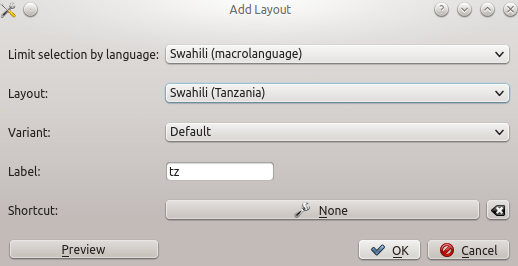
\includegraphics[keepaspectratio=true]{./images/kdelg.png}
% kdelg.png: 518x266 pixel, 96dpi, 13.70x7.04 cm, bb=0 0 388 199
\caption{Setting up the Swahili keyboard for KDE}
\label{fig:kdelg}
\end{figure}

Click \textbf{OK}, and then \textbf{Apply} to exit.

You should now see an additional marker in the system tray at the bottom right of your screen, which will be the abbreviation for the default language on your desktop.  For instance, if you have UK English as the default, you will see \textbf{gb}.  Click on this, and it will change to \textbf{tz}, showing that the keyboard for Swahili in Arabic script is now operational.  You can quickly switch between the two keyboards by pressing \textbf{Ctrl+Alt+K}.

Close the \textit{System Settings} box.

Note that if you make changes to the keyboard layout, you need to re-apply the layout -- see the end of \Cref{appC}.

\subsection{Activate the new keyboard in Unity}

If you have decided to stick to Unity as your desktop, click the \textbf{System Settings} icon in the Launcher, or click the system icon in the top right-hand corner and select \textbf{System Settings}.

Click \textbf{Text entry} in the \textit{Personal} section.

Click on the + at the bottom of the left-hand pane, \textit{Input sources to use}.

Roll down to \textit{Swahili (Tanzania)}.

Click on it and then click \textbf{Add}.

Close the \textit{Text entry} box.

There should be a new icon on the menu bar.  Either Click on the language chooser icon on the menu bar and choose Swahili from the list.  Alternatively, press \textbf{Super} (usually the key with a Windows logo on it) \textbf{+ Space}.

\subsection{Interaction with the unlock screen in KDE}

If you have the unlock screen activated, this means that when you leave your machine for some time, it will power down the screen and then, when you resume work, present a login box so that you can unlock the desktop.   A problem arises if you changed the  keyboard to Swahili before leaving your machine -- since the machine was powered down with that keyboard active, the login box will only allow you to type Arabic glyphs, which means that you cannot type in your (Roman glyph) password!

The easiest way to deal with this is to disable the unlock screen by going to \textbf{K} \textrightarrow\ \textbf{Settings} \textrightarrow\ \textbf{System Settings \textrightarrow\ Power Management \textrightarrow\ Advanced Settings}, and unticking \textit{Lock screen on resume}.

If for some reason you wish to retain the lock screen, you can recover from this situation whenever it occurs by pressing \textbf{Crtl+Alt+F5} to get a terminal login.  Type your username and password to log in.

Open the configuration file for the keyboard:\\
\verb|nano ~/.kde/share/config/kxkbrc|

Find the line:\\
\verb|LayoutList=gb,tz|\\
and change it to:\\
\verb|LayoutList=gb|

Save the file: \textbf{Ctrl+X, Y, Return}.\\
(The example here uses the UK English keyboard, \textit{gb} -- replace this with whatever your own default keyboard is.)

Press \textbf{Ctrl+Alt+F7} to return to the unlock screen.  Click the login box, and you should be able to login as normal.  However, you will need to re-add the Swahili keyboard as shown above.


\section{LibreOffice}
\label{s:libreoffice}

LibreOffice, installed by default in Ubuntu, is a suite of office software (word processor, spreadsheet, presentation program, etc).  The version used here is 4.2.4.2.

\subsection{Configure the word-processor}

Open LibreOffice Writer.

Click on \textbf{Tools \textrightarrow\ Options \textrightarrow\ Language Settings \textrightarrow\ Languages}.

Under \textit{Default languages for documents}, tick \textbf{Complex text layout (CTL)}, and select \textbf{Arabic (Oman)} in the dropdown.  Click OK.

Click on \textbf{Tools \textrightarrow\ Options \textrightarrow\ Language Settings \textrightarrow\ Complex Text Layout}.

If you wish to use both Arabic-Indic numerals (on the numeral keys) and Western-Arabic numerals (AltGr+numeral), ensure Arabic or System is chosen here. The other two settings will convert Western-Arabic numerals to their Arabic-Indic equivalents.

Tick \textbf{Visual} under \textit{Cursor control}, and then \textbf{OK}.

Right-click on the toolbar, and under \textit{Visible buttons} select \textbf{LTR}.  Do the same to select \textbf{RTL}.  Two new buttons will now appear in the Formatting toolbar, one for left-to-right typing, and one for right-to-left typing.

Shortcuts are \textbf{Ctrl+Shift+A} for LTR and \textbf{Ctrl+Shift+D} for RTL.

\subsection{Install a template}

Andika! includes in \textit{andika/libreoffice} a template (\textit{andika.ott}) where styles for Swahili in Arabic script, Swahili in Roman script (standard spelling or close transcription) and translation are already set up -- all these styles are right-justified.  Installing the template is optional, but it will make typing out Swahili poetry much simpler.

Click on \textbf{File \textrightarrow\ Templates \textrightarrow\ Manage}.

On the \textit{Documents} tab, double-click \textbf{My Templates} and then click \textbf{Import}.

Navigate to \textit{andika/libreoffice/andika.ott} and click on it -- it should now be listed there as a template.

If you want to set it as the default (nothing has been changed from the stock default apart from the addition of the three extra styles), click on it and then click \textbf{Set as default}.

To use the template without setting it as default, select \textbf{File \textrightarrow\ New \textrightarrow\ Templates \textrightarrow\ andika}.

Close the \textit{Templates} box, and then restart LibreOffice Writer.

To use the styles, place the cursor in the line you wish to format, press \textbf{F11} to open the \textit{Styles and Formatting} list, and select the relevant style by double-clicking on its name -- the new styles are at the bottom of the list.

\textit{Arabic} style is RTL, Scheherazade 24pt.  You may wish to make the font size smaller. In unvocalised Arabic, reading the text is possible at quite small font sizes. In Swahili, however, the vowel signs are essential, so the same reductions in font size are not possible.  In typesetting poetry, the lines are usually short, and accuracy is improved by having a large font size.

\textit{Roman} style is LTR, right-justified, Liberation Serif 12pt.

\textit{Translation} style is LTR, right-justified, Liberation Serif 12pt, italic.  

Obviously, the appropriate writing system (Arabic or Roman) also has to be selected on the keyboard before typing (see \Cref{s:keyboard}).


\section{PHP}

PHP is a computer language which is used to convert text from one script to the other, and also for the import and export of text to and from the database.

\subsection{Install PHP}

\verb|sudo apt-get install php5 php5-cli|

To test the install:\\
\verb|php --version|\\
(note: two dashes)\\
You should get a message giving details about the version of PHP you've just installed.

\subsection{Configure PHP}

\verb|sudo nano /etc/php5/cli/php.ini|

This command will open the system file \textit{php.ini} in a lightweight text editor called \textit{nano}, where you have to change some settings.  Use the arrow keys on the keyboard to move around, and the Home and End keys to move to the beginning or end of a line.

Press \textbf{Ctrl+W}, then type\\
\verb|max_execution_time|\\
into the searchline and press \textbf{Return}. Change the line to read:\\
\verb|max_execution_time = 300|

Again press \textbf{Ctrl+W}, type\\
\verb|error_reporting| \\
and press \textbf{Return}. Change that line to: \\
\verb|error_reporting = E_ALL & ~E_NOTICE & ~E_DEPRECATED|

A bit lower down from that (you can scroll down using the mouse), there is a \textit{display\_errors} line. Change it to read: \\
\verb|display_errors = On|

Below that there is a \textit{log\_errors} line. Change it to read: \\
\verb|log_errors = Off|

To save the file, press \textbf{Ctrl+X}, then press \textbf{Y} to confirm you want to save the modifications, and press \textbf{Return} to close the file.


\section{PostgreSQL}

PostgreSQL is a database which is used to store the words of the text for editing and enhancement.


\subsection{Install PostgreSQL}

\verb|sudo apt-get install postgresql postgresql-client postgresql-common|

$\hookrightarrow$ \verb|postgresql-contrib php5-pgsql|

To test the install:\\
\verb|psql|

You should get an error message saying that the role named after your username does not exist.


\subsection{Set up a database user}
\label{ss:dbuser}

On Ubuntu, PostgreSQL uses peer authentication by default.  This means that creating a database user with the same name as your system (Ubuntu) user will mean you can log in to the database without entering a password.\footnote{If for security reasons you wish to enter a password each time your user accesses a database, open the configuration file: \texttt{sudo nano /etc/postgresql/9.3/main/pg_hba.conf}.  Find the line: \texttt{local all all peer} and change it to read \texttt{local all all md5}.  Save the file: \textbf{Ctrl+X, Y, Return}.  Restart PostgreSQL: \texttt{sudo service postgresql restart}.  You will now need to enter your database password even to connect to the database under your system username.}  The terminal prompt should tell you what your username is -- it is of the form \textit{user@computer}.  Alternatively, you can run:\\
\verb|whoami|\\
to find out your username.

\verb|sudo -i|

The prompt will change to show that you are now \textit{root} (the superuser, or administrator).

\verb|su - postgres|\\
(note the space on either side of the dash)

The prompt will change to show that you are now the \textit{postgres} master user.

Create a new database user with the same name as your system user (replace USER with your system username):\\
\verb|createuser -P -s -e USER|

You will be asked to enter a password -- note that you will get no feedback (the line will stay blank).  Press \textbf{Return} and you will be asked to enter the password again.  Press \textbf{Return} and you should get a message beginning \textit{CREATE ROLE}, meaning that the new user has been created.

\verb|exit|\\
to cease being the postgres user.

\verb|exit|\\
to cease being the superuser.


\subsection{Set Andika! to use your database user}

\verb|nano andika/config.php|

Change:\\
\verb|user=kevin password=kevindbs|\\
to read:\\
\verb|user=USER password=yourpassword|\\
and save the file (\textbf{Ctrl+X, Y, Return}).

Remember to replace USER with your username.


\subsection{Create the andika database}

\verb|createdb andika|

This creates the \textit{andika} database, owned by your new user.

\textbf{Andika!} comes with starter data in \textit{andika/db/starter/andika.sql}, which can be imported into the new database:\\
\verb|psql -d andika < db/starter/andika.sql|

If you chose a username other than \textit{dbmaster}, use that instead.


\subsection{Connect to the \textit{andika} database}
\label{ss:connect}

\verb|psql -d andika|

The prompt should change to \textit{andika=\#}. 

\verb|\dt|\\
(= display tables)

This should show a list with 18 rows, each representing a database table holding poem information in the \textit{andika} database.  To look at the table for the poem \textit{kiswahili}:

\verb|select * from kiswahili;|\\
(note: the semicolon at the end is an integral part of the command)

This will show everything in the \textit{kiswahili} table.  Exit the data display and go back to psql:\\
\verb|q|

To see something more selective:\\
\verb|select * from kiswahili where stanza=1 order by stanza, loc;|\\
(again, remember the semicolon at the end)

You should get a listing of the \textit{vipande} in the first stanza of the poem \textit{Kiswahili} from the Abdulkadir and Frankl paper, in order of \textit{kipande}.  Exit the data display and go back to psql:\\
\verb|q|

\verb|\q|\\
to exit \textit{psql}.


\section{Database interfaces}

To make it easier to read and edit the contents of the PostgreSQL database, it is best to install an interface.  Two of these will be installed, each differing in their capabilities.  The first is a web-based interface called phpPgAdmin, which first requires a webserver (Apache) to be installed.  The second interface is called SQL Workbench, and it requires a computing language called Java to be installed.

\subsection{phpPgAdmin}

\subsubsection{Install Apache}
\label{ss:apache}

\verb|sudo apt-get install apache2 apache2-utils phppgadmin|

Start the webserver:\\
\verb|sudo service apache2 start|

If you want to get rid of the (harmless) message \textit{Could not reliably determine the server's fully qualified domain name, using 127.0.1.1. Set the `ServerName' directive globally to suppress this message}, issue the following commands:\\
\verb+echo "ServerName localhost" | sudo tee /etc/apache2/conf-available/servername.conf+\\
\verb|sudo a2enconf servername|\\
\verb|sudo service apache2 restart|

Test the install -- open a web browser (preferably Firefox) and type:\\
\verb|http://localhost|\\
into the address bar. A page should open, telling you that Apache is installed and working.

\subsubsection{Configure phpPgAdmin}

Activate the phpPgAdmin configuration file:\\
\verb|sudo cp /etc/apache2/conf.d/phppgadmin /etc/apache2/conf-enabled/phppgadmin.conf|

Restart the webserver:\\
\verb|sudo service apache2 restart|

In the web browser, type\\
\verb|http://localhost/phppgadmin|\\
into the address bar.

You should see the phpPgAdmin homepage. On the left side there is a list of servers (in this case, there should only be one listed). Click on \textbf{PostgreSQL} and you should get a login form.

Fill in the username and password for PostgreSQL (which you created in \Cref{ss:dbuser}) and click \textbf{Login}.

The default session time for PHP is set to 24 minutes (1440 seconds).  This means that if you do not use phpPgAdmin for 24 minutes, it will ask you to log in again before you can continue using it.  If you find that this interrupts your workflow, you can change the setting in the PHP configuration file:\\
\verb|sudo nano /etc/php5/apache2/php.ini|

Press \textbf{Ctrl+W}, then type:\\
\verb|session.gc_maxlifetime|

and press \textbf{Return}. Change the line to read: \\
\verb|session.gc_maxlifetime = 144000|

This will allow you 40 hours before logging you out, which should be sufficient.

\subsubsection{Test phpPgAdmin}
\label{ss:testppa}

In the left-hand panel you should get a list of your current databases -- there should only be two: \textit{andika} and the system database \textit{postgres}. (The right-hand panel shows you the same two databases.)

Click the \textbf{+} beside \textit{andika} in the left-hand panel.  It should open to show \textit{Schemas, public, Tables} etc. Click on \textbf{Tables}. The right-hand panel should now show you all the tables inside the \textit{andika} database, similar to what you saw in Section \ref{ss:connect}.

Click on \textbf{kiswahili} and you will see the data fields in that table. To see the contents of the database you can click on the \textbf{Browse} button.

To see the data fields of each item in more detail, click on the \textbf{Edit} button beside each row in the table -- changes to the fields can be made and saved here.

To make a database query, click the \textit{SQL} link at the top right of the phpPgAdmin window.  This will open another smaller window.  In the large textbox, type:\\
\verb|select * from kiswahili where stanza=1 order by stanza, loc;|\\
(again, remember the semicolon at the end)

Click Execute, and in the first window you should see a listing of the \textit{vipande} in the first stanza of the poem, in order of \textit{kipande}, as you did in Section \ref{ss:connect}.  In this case, though, the contents are a lot easier to read!


\subsection{SQL Workbench}
\label{ss:workbench}

\subsubsection{Install Java}

Andrei Alin\footnote{\url{webupd8.org}} maintains links to up-to-date versions of Java in his software repository.

Check that the helper script \textit{add-apt-repository} is installed:\\
\verb|sudo apt-get install software-properties-common|

Add the new software repository:\\
\verb|sudo add-apt-repository ppa:webupd8team/java|

Update the software package lists to include software from the new repository:\\
\verb|sudo apt-get update|

Install the Java installer:\\
\verb|sudo apt-get install oracle-java8-installer|

This installs a script that then downloads and installs Oracle Java 8 -- it may therefore take a few minutes.  To test the install:\\
\verb|java -version|\\
This should return some text telling you that the Java version is 1.8.0.

Set the Java environment variables:\\
\verb|sudo apt-get install oracle-java8-set-default|

\subsubsection{Install JDBC}
\label{ss:jdbc}

JDBC (Java DataBase Connector) is a driver which will allow SQL Workbench to connect to the PostgreSQL database.

\verb|sudo apt-get install libpostgresql-jdbc-java|

\subsubsection{Install SQL Workbench}

Create a directory to hold the files:\\
\verb|mkdir sqlworkbench|

Go to the website \textit{sql-workbench.net}, click on the link for \textit{Build 116} (or whatever the current stable version is), and download the generic package.  Save it in the \textit{andika} directory.

Unzip the download into the new directory:\\
\verb|unzip -q Workbench-Build116.zip -d sqlworkbench|

Make the launch script executable:\\
\verb|chmod +x sqlworkbench/sqlworkbench.sh|

Launch SQL Workbench:\\
\verb|sqlworkbench/sqlworkbench.sh|

If you wish, you can make a desktop shortcut or menu entry to make launching SQL Workbench easier.

\subsubsection{Configure SQL Workbench}

A \textit{Select Connection Profile} box should come up. 

Change \textit{New profile} to read \textbf{andika}.

Click the drop-down arrow on the \textit{Driver} line and select \textit{PostgreSQL}. Click \textbf{Yes}, when you're asked whether you want to edit the driver definition.

On the \textit{Manage Drivers} popup, click on the red \textit{postgresql} entry already there and then click X to delete it.  Click on the folder icon and navigate to \textit{/usr/share/java/postgresql-jdbc4-9.2.jar} (which you installed in Section \ref{ss:jdbc}.  Click \textbf{Open}, and then \textbf{OK}.

Check that the \textit{URL} line reads \textit{jdbc:postgresql://localhost:5432/andika} -- if not, edit it to make it so. Enter your PostgreSQL username and password (Section \ref{ss:dbuser}), and then click \textbf{OK}.  You should get a connecting message.

\subsubsection{Test SQL Workbench}

The main screen consists of a top pane where you type database queries, and a bottom pane where the results will appear. 

In the top pane, type:\\
\verb|select * from kiswahili where stanza=1 order by stanza, loc;|\\
(remember: the semicolon at the end is an integral part of the command)

Move the cursor somewhere in the middle of that query and press \textbf{Ctrl+Return}.  In the bottom pane, you should see a listing of the \textit{vipande} in the first stanza of the poem, in order of \textit{kipande}, as you did in Sections \ref{ss:connect} and \ref{ss:testppa}.

The main benefit of SQL Workbench compared to phpPgAdmin is that a result set can be directly edited -- this makes it easy to add data.  To try this, select one of the cells under the \textit{english} column, type something in, and press \textbf{Return}.  A yellow diamond will appear in the leftmost column, showing that the record has been edited but not saved yet. To save it you need to click the disk icon, or select \textbf{Data \textrightarrow\ Save changes to database} and click \textbf{OK} when asked to confirm.

You can check the change was made by running the same query in phpPgAdmin's SQL box (see Section \ref{ss:testppa}) :\\
\verb|select * from kiswahili where stanza=1 order by stanza, loc;|

To delete the change, click the cell in SQL Workbench, press \textbf{Backspace} and then \textbf{Return}, and then save as before.

Close SQL Workbench, clicking Yes to save the new \textit{andika} connection profile you have set up.


\section{LaTeX}
\label{s:latex}

LaTeX is a typesetting system that is capable of creating very complex layouts.  It is used in \textbf{Andika!} to provide attractive output.

\verb|sudo apt-get install texlive texlive-xetex texlive-generic-extra texlive-humanities|\\
$\hookrightarrow$ \verb|texlive-lang-arabic texlive-latex-extra texlive-bibtex-extra kile kbibtex biber|

Note that these packages will take perhaps 20 minutes to download and install.


\section{JabRef}
\label{s:jabref}

JabRef\footnote{jabref.org} is a bibliography manager.

\verb|sudo apt-get install jabref|


\section{YAD}

YAD (Yet Another Dialogue),\footnote{\url{sourceforge.net/projects/yad-dialog/}} maintained by Victor Ananjevsky, is used by \textbf{Andika!} to provide a point-and-click interface to the conversion script.  To install it, we need to add another of Andrei Alin's\footnote{\url{webupd8.org}} repositories.

Add the new software repository:\\
\verb|sudo add-apt-repository ppa:webupd8team/y-ppa-manager|

Update the software package lists to include software from the new repository:\\
\verb|sudo apt-get update|

Install YAD:\\
\verb|sudo apt-get install yad|\footnote{You may also wish to install Andrei's own Y-PPA-Manager -- \texttt{sudo apt-get install y-ppa-manager}.  This is not used by \textbf{Andika!}, but is a very useful system tool to keep track of the software repositories on your machine.}


\section{Access the \textit{Andika!} website locally}
\label{s:localaccess}

Although not essential to use \textbf{Andika!}, it may be useful to have access to a local copy of the website (\textit{kevindonnelly.org.uk/swahili}).  

First, tell the webserver installed earlier (Apache -- see Section \ref{ss:apache}) where to find the\textbf{ Andika!} webpages.

Open a configuration file:\\
\verb|sudo nano /etc/apache2/sites-available/andika.conf|

Type the following lines into the file:\\
\vspace{-0.5cm}  % get rid of the excess space before the verbatim environment
\begin{verbatim}
<VirtualHost *:80>
ServerName andika
DocumentRoot /var/www/andika/
</VirtualHost>
\end{verbatim}

Save and exit the configuration file:\\
\textbf{Ctrl+X, Y, Return}

Activate the configuration:\\
\verb|sudo a2ensite andika|

Restart the webserver:\\
\verb|sudo service apache2 restart|

Then tell your web browser that the new website is on your machine, so it doesn't have to look for it on the web.

Open a configuration file:\\
\verb|sudo nano /etc/hosts|

After the line:\\
\verb|127.0.0.1	localhost|\\
add the following line:\\
\verb|127.0.0.1	andika|

Save and exit the configuration file:\\
\textbf{Ctrl+X, Y, Return}

In a web browser, type:\\
\verb|http://andika/index.php|\\
into the address bar.  You should get the \textbf{Andika!} website loading from the files on your hard disk (in \textit{/var/www/andika}), instead of from the internet.


